\pagebreak

\section{Introduction}
\label{sec:introduction}

\paragraph{}The main objective of this final laboratory assignment is to design and study a bandpass filter, using various components, such as the 741 OP-AMP, resistors and capacitors, while, at the same time, trying to maximize our figure of merit M.

\paragraph{}
In Section~\ref{sec:theoretical}, a theoretical introduction is made in order to contextualize all the main principles that sustain our construction and analysis of the circuit. A theoretical Bandpass Filter circuit is built and carefully analysed in Section~\ref{analysis}, where the results are obtained in GNU Octave. Also, in Section~\ref{sec:simulation}, the Bandpass Filter circuit is analysed by simulation through the use of NGSpice to simulate the real electric circuit behaviour. The results of the simulation of Section~\ref{sec:simulation} are then compared to the theoretical results obtained in Section~\ref{analysis} and the comparative results are expressed in Section~\ref{error}. The figure of merit, calculated according to the components used to build the simulation circuit, can also be found in Section~\ref{error}. The conclusions of this study are outlined in the final part of the report, in Section~\ref{sec:conclusion}.

\begin{figure}[H] \centering
	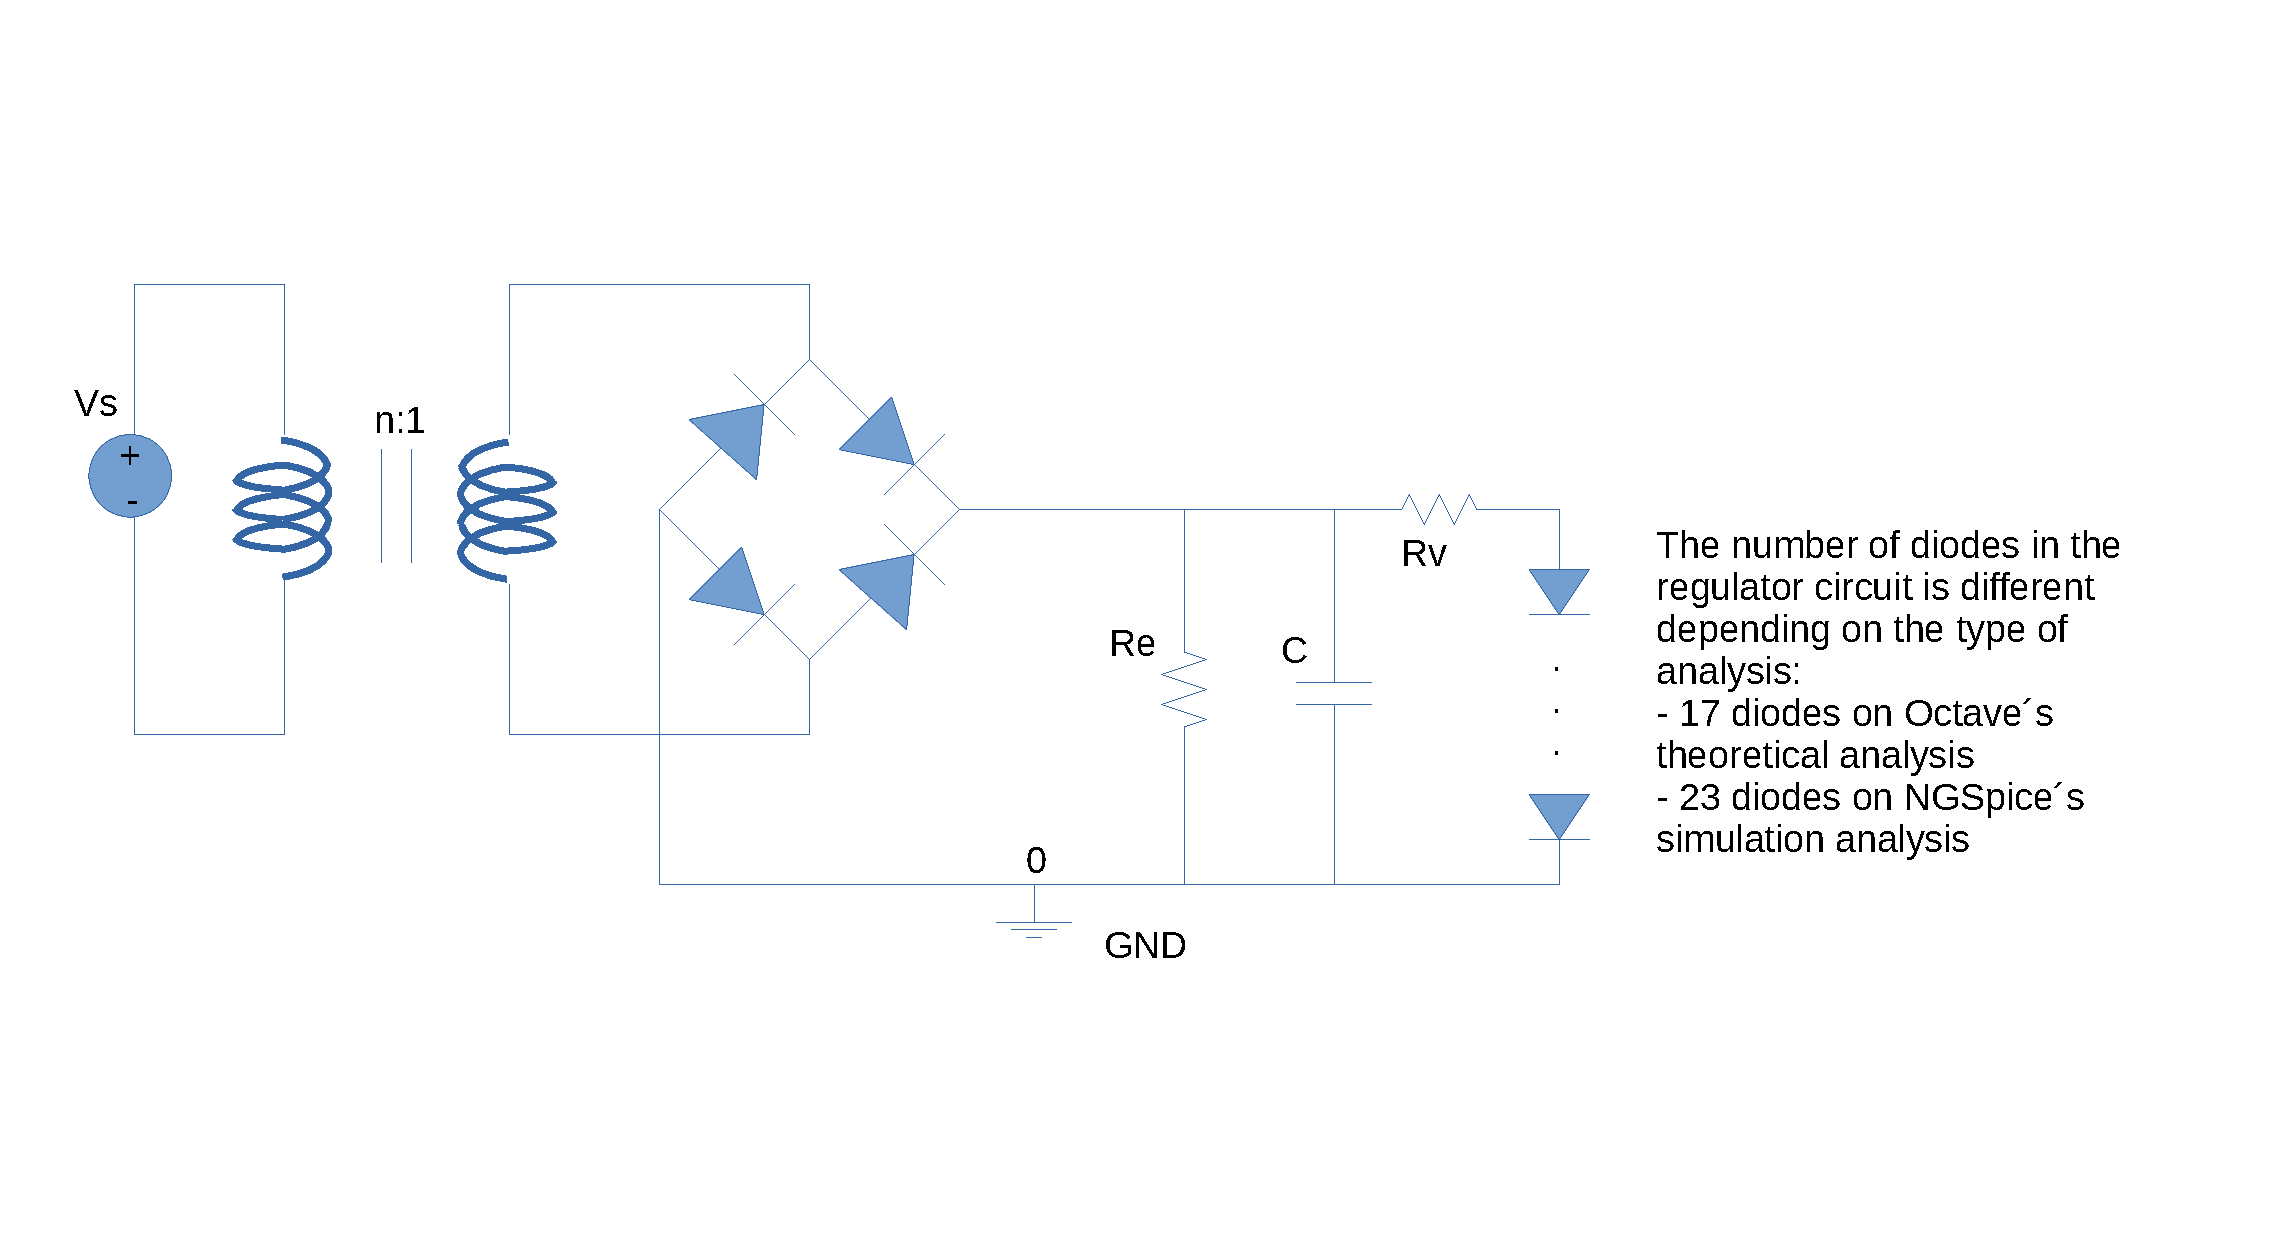
\includegraphics[width=0.7\linewidth]{circuit.pdf}
	\caption{Fifth laboratory circuit.}
	\label{fig:circuit}
\end{figure}
